\documentclass{article} 

%\documentclass{article}

% Language setting
\usepackage[english]{babel}

% Set page size and margins
% Replace `letterpaper' with `a4paper' for UK/EU standard size
\usepackage[letterpaper,top=2cm,bottom=2cm,left=3cm,right=3cm,marginparwidth=1.75cm]{geometry}

% Useful packages
\usepackage{amsmath}
\usepackage{graphicx}
\usepackage[x11names]{xcolor}
\usepackage[colorlinks=true, citecolor=magenta, linkcolor=black]{hyperref}
\usepackage{authblk}
\usepackage{blindtext}
\usepackage{multicol}
\usepackage{float}
\usepackage{subcaption}


\newcommand\C[1]\null


\title{\bf{Distinguishing Between Cosmic Strings and Glitches in Gravitational-Wave Data Using a Neural Network}}
\author[1]{Marlinde Drent}
\author[1]{Marc Duran Gutierrez}
\author[1]{Bo Ribbens}

\affil[1]{\it{Department of Physics, Utrecht University}}

\begin{document}
\maketitle

% Maybe add abstract?
\begin{abstract}
    The detection of cosmic strings is important because reasons \C{why do we want them?}. 
    The search for these comsic strings is being held back by detector glitches.
    These glithces can strongly resemble comsic strings. 
    It is therefore very important to develop a method of distinguishing between a cosmic string signal and a glitch.
    In the work we focus on using a neural network for this task.
\end{abstract}

\begin{multicols}{2}
\section{Introduction}
% A very general introduction
The first detected gravitational wave (GW) signal was GW150914\cite{PhysRevLett116061102} in 2015. 
These GW signals can originate from several sources, one of which is cosmic strings.
Since the first observed GW many technological advancements have been made, yet one thing that still plagues detectors is the presence glitches.    
These are bursts of non-Gaussian noise that look like a signal \C{Needs citation}.
These glitches can be mistaken for a signal, so it is important to find a way to distinguish between a signal and a glitch.
In this work we focus on the use of machine learning to distinguish between a glitch and a signal.

\subsection{Cosmic strings and glitches}
% A deep dive into cosmic srings
Cosmic strings are one-dimensional topological defects and originate form field theories~\cite{Meijer_2024}.
These defects could have formed from spontanious symmetry breaking in the early universe~\cite{schmitz2024gravitationalwavescosmicstrings}.
These cosmic strings are of interest since they affect our understanding of physics, and can help confirm or rule out centrain physics models. \\
\indent
Cosmic strings appear at cosmological scales as thin strings with large densities, and their motion is well described by the Nambu-Goto action~\cite{MairiSakellariadou}.
Cosmic stings can both be open strings or closed loops, and two cosmic strings are able to interact with eachother. \C{Needs citation}\\
\indent
To detect cosmic strings we first need to understand what a GW signal with a cosmic string source looks like.
Cosmic strings can produce GW signals in multiple ways. Examples include the formation of cusps and kinks~\cite{PhysRevLett126241102}. 
Here we will focus on the cusps. A cusp is a singularity, where a point traveling along the curve would have to turn around.
When this occurs, the physical string snaps into a cusp shape, and is instantaniously accelerated to the speed of light at that point.
A burst GW is then emitted in the direction of acceleration~\cite{Meijer_2024}.
Such a signal can be seen in the left plot in figure~\ref{CS_signal_and_glitch}.\\
\begin{figure}[H]
    %Here I want both the signal and the glitch plot, side by side
    \centering
    \begin{subfigure}[b]{0.49\columnwidth}
        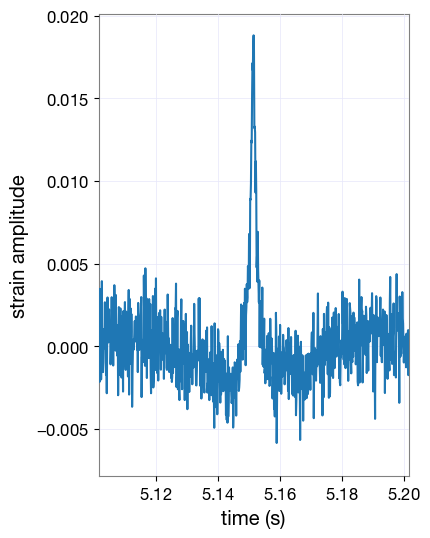
\includegraphics[width=\linewidth]{../Dataplots/injection3.png}
        \caption{The signal produced by the cusp of a cosmic string.}
    \end{subfigure}
    \hfill
    \begin{subfigure}[b]{0.49\columnwidth}
        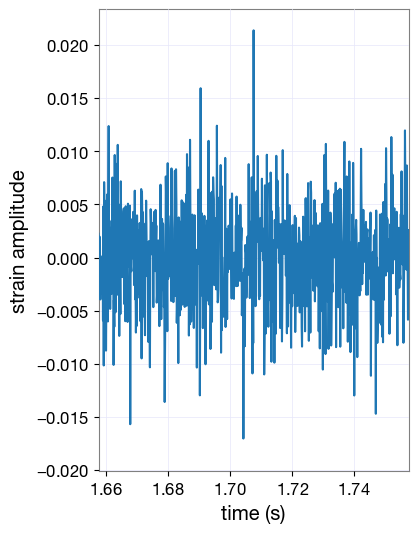
\includegraphics[width=\linewidth]{../Dataplots/background3.png}
        \caption{Background noise with a peak.}
    \end{subfigure}
    \caption{The signal and glitch plots side by side.}
    \label{CS_signal_and_glitch}
\end{figure}
\indent
Whith the knowledge of what the signal looks like, the next step is to search for a signal.
The problem with this is that the form of the signal is very similar to that of centrain glitches, like the blip glitch.
Blib glitches are short noise transients with a large frequency bandwidth~\cite{Cabero_2019}. 
The form of this glitch can be seen in the right plot in figure figure~\ref{CS_signal_and_glitch}\\
\indent
Since a GW signal from cosmic strings can be so similar to glitches, it is crucial to develop a method to distinguish between them.

\subsection{Machine learning}
% explain what machine learning is


\section{Method}
\subsection{Data}
% explain the data structure

\subsection{Neural network structure}
% explain the neural network structure (inlcude figure)

\indent
The proposed model used in this work is a convolutional neural network (CNN) designed for a bianry classification problem.
The architecture, shown is Fig. X, extracts features from the input through seven convolution layers, 
followed by a fully conected layers that classify the input as either a signal peak or background noise.
The network accepts three initial time series, coming from three diferent telescopes, which are transformed into a feature map by convolving them.
This input data can be represented as a 3D tensor with shape (T, 1, 3) where T is the lenght of the time series,
1 is a single channel for each time step, and 3 denotes the number of imput features corresponding to the three telecopes.

After passing through a convolutional layer, the data is modified by the appliaction of a specfic chosen number N of kernels (also called filters).
the kernels used have a shape of (k, input channels) with ks ranging from 3 to 7 (idk have to check.).

The kernels slide over the time axis of the input data, performing element-wise multiplications and then summing the elements. 
This produces a diferent feature map for each kernel which encodes specific patterns or correlations over the window defined by k.

The resulting ouput tensor has a shape (T', number of features map). T' is the length of the time axis after convolution, 
which depends on the kernel size, stride, and padding.







\section{Results}
\subsection{Accuracy}
% Show the accuracy of the neural network (include plot)

\subsection{Efficiency}
% Plot of loss and validation
% Some facts on the loss, training loops, time taken, etc.


\section{Discussion}
% Suggestions for further research -> how to improve the NN?


\section{Conclusion}
%TO DO:
% Conclude if NN works

\bibliographystyle{unsrt}
\bibliography{Cosmic_report}
\end{multicols}
\end{document}



%\begin{figure}
%\centering
%\includegraphics[width=0.25\linewidth]{}
%\caption{\label{fig:frog}This frog was uploaded via the file-tree menu.}
%\end{figure}